\documentclass[12pt, letterpaper]{article}

% --- PACKAGES ---
\usepackage[margin=1in]{geometry}  % 1-inch margins
\setlength{\headheight}{14.49998pt} % Fix fancyhdr warning
\setlength{\parindent}{0pt}        % Remove paragraph indentation
\setlength{\parskip}{0.5em}          % Add space between paragraphs
\usepackage{amsmath, amssymb, amsfonts} % For math equations 
\usepackage{graphicx}              % For including plots 
\usepackage{fancyhdr}              % For headers/footers
\usepackage{hyperref}              % For clickable links (e.g., to figures)
\usepackage{listings}              % For formatting code 
\usepackage{float}                 % For better figure placement (e.g., [H])
\usepackage{caption}               % For figure captions
\usepackage{subcaption}            % For subfigures with subcaptions
\usepackage{xcolor}                % For defining colors in listings
\usepackage{pdfpages}              % For including PDF files
\usepackage{tikz}                  % For creating diagrams
\usetikzlibrary{shapes.geometric, arrows.meta, positioning, fit, backgrounds}
\usepackage[ruled,vlined]{algorithm2e} % For pseudocode algorithms

% --- LISTINGS (CODE) SETUP ---
% Define a style for Julia code
\definecolor{codegreen}{rgb}{0,0.6,0}
\definecolor{codegray}{rgb}{0.5,0.5,0.5}
\definecolor{codepurple}{rgb}{0.58,0,0.82}
\definecolor{backcolour}{rgb}{0.98,0.98,0.98}

% Define a basic Julia language for listings so 'language=Julia' is recognized.
% This provides common keywords, comment and string delimiters.
\lstdefinelanguage{Julia}{
    keywords={function,end,for,while,if,else,elseif,return,break,continue,struct,mutable,using,import,export,let,global,local,const,macro},
    sensitive=true,
    morecomment=[l]{\#},
    morestring=[b]"
}

\lstdefinestyle{julialang}{
    backgroundcolor=\color{backcolour},   
    commentstyle=\color{codegreen},
    keywordstyle=\color{blue},
    numberstyle=\tiny\color{codegray},
    stringstyle=\color{codepurple},
    basicstyle=\ttfamily\footnotesize,
    breakatwhitespace=false,         
    breaklines=true,                 
    captionpos=b,                    
    keepspaces=true,                 
    numbers=left,                    
    numbersep=5pt,                  
    showspaces=false,                
    showstringspaces=false,
    showtabs=false,                  
    tabsize=2,
    language=Julia,
    % {<char>}{<LaTeX code>}{<length>}
    literate={θ}{{$\theta$}}1
             {Δ}{{$\Delta$}}1
             {ν}{{$\nu$}}1
             {π}{{$\pi$}}1
}
\lstset{style=julialang} % Apply this style by default

% --- HEADER/FOOTER ---
\pagestyle{fancy}
\lhead{Grid Generation via Frame Fields}
\rhead{Marvyn Bailly}
\cfoot{\thepage}

% --- TITLE INFORMATION ---
\title{Automatic Structured Quadrilateral Grid Generation via Frame Fields} % 
\author{Marvyn Bailly}
\date{December 11, 2025} 


\begin{document}

\maketitle
\thispagestyle{empty} % No header/footer on the title page

% --- ABSTRACT ---
\begin{abstract}
This paper presents an investigation into automatic structured quadrilateral grid generation using frame fields. The research explores the theoretical foundations and practical implementation of frame field-based methods for generating high-quality structured meshes suitable for finite volume methods. We discuss the mathematical framework, implementation details, and demonstrate the effectiveness of the approach through various test cases.
\end{abstract}

\vspace{0.5in}

\clearpage

% --- TABLE OF CONTENTS ---
\tableofcontents
\clearpage

% --- INTRODUCTION ---
\section{Introduction}

In Computional Fluid Dynamics (CFD), the generation of high-quality meshes is crucial for accurate simulations which use finite volume methods. Structured quadrilateral grids are particularly advantageous due to their regular connectivity and alignment with flow features. This paper explores the use of frame fields for automatic generation of structured quadrilateral grids, providing a systematic approach to mesh generation that can adapt to complex geometries. In this study, we implement the Mixed-Integer Quadrangulation (MIQ) method in Julia as described by Bommes et al. (Bommes 2009) and evaluate its performance on various geometries. 

We aim to generate structured quadrilateral meshes that maintain the following qualities:
\begin{itemize}
    \item \textbf{Indiviual Cell Quality:} Each quad should be as close to a square as possible. 
    \item \textbf{Orientation:} The grid should align with the geometry's features and flow directions.
    \item \textbf{Alignment:} The grid should resolve sharp features and boundaries accurately.
    \item \textbf{Global Structure:} Points in the mesh known as singularities are required to composite for the Gaussian curvature of a general surface. singularities correspond to irregular vertices in the quad mesh where the number of incident edges differs from four. These should be minimized and strategically placed.
\end{itemize}
In the following sections, we will detail the methodology used to implement the MIQ algorithm, present the results of our mesh generation experiments, discuss the implications of our findings, and conclude with insights in this area.




% --- METHODOLOGY ---
\section{Methodology}
We break the methodology into two main steps: (1) Frame Field Generation and (2) Quadrilateral Mesh Extraction. The core of both steps relies on solving a minimzation problem where some of the variables are integers while the others are real-valued. This is known as a Mixed-Integer Program (MIP) which are generally NP-hard to solve. To address this, we implement an approximation algorithm known as a greedy mixed-integer solver as described by Bommes et al.. 

\subsection{Mixed-Integer Solver}

\subsubsection{Problem Formulation}

The minimzation of a quadratic energy function $E(x_1, \dots, x_n)$ is an integer problem if $x \in \mathbb{Z}^n$. However, in this paper, we encounter a more general problem were some of the unknown variables $x_1, \dots, x_k$ are integers while the remaining variables $x_{k+1}, \dots, x_n$ are real-valued. This is known as a Mixed-Integer Program (MIP) which are generally NP-hard to solve and so we hope to avoid solving them directly. We note that the continuous relaxation of a MIP, obtained by allowing all variables to be real-valued, provides a lower bound on the optimal solution of the original MIP. Thus this provides a reasonable starting point for approximation algorithms.

\subsubsection{Common Approaches}
A common approach to approaching a MIP is to first compute the continuous minimizer, which simlpiy requires the solution of the linear system $\{ \partial E / \partial x_i = 0 \}_{i=1}^n$. Then the first $k$ variables of the oslution are rounded to the nearest integer and treated as constant while resolving the linear system for the remaining real-valued variables. This is known as direct rounding but the solution can signficailty deviate from the optimal solution. This motivates the authers to propose a greedy mixed-integer solver which is explained next.

\subsubsection{Greedy Mixed-Integer Solver}
\begin{figure}
\centering
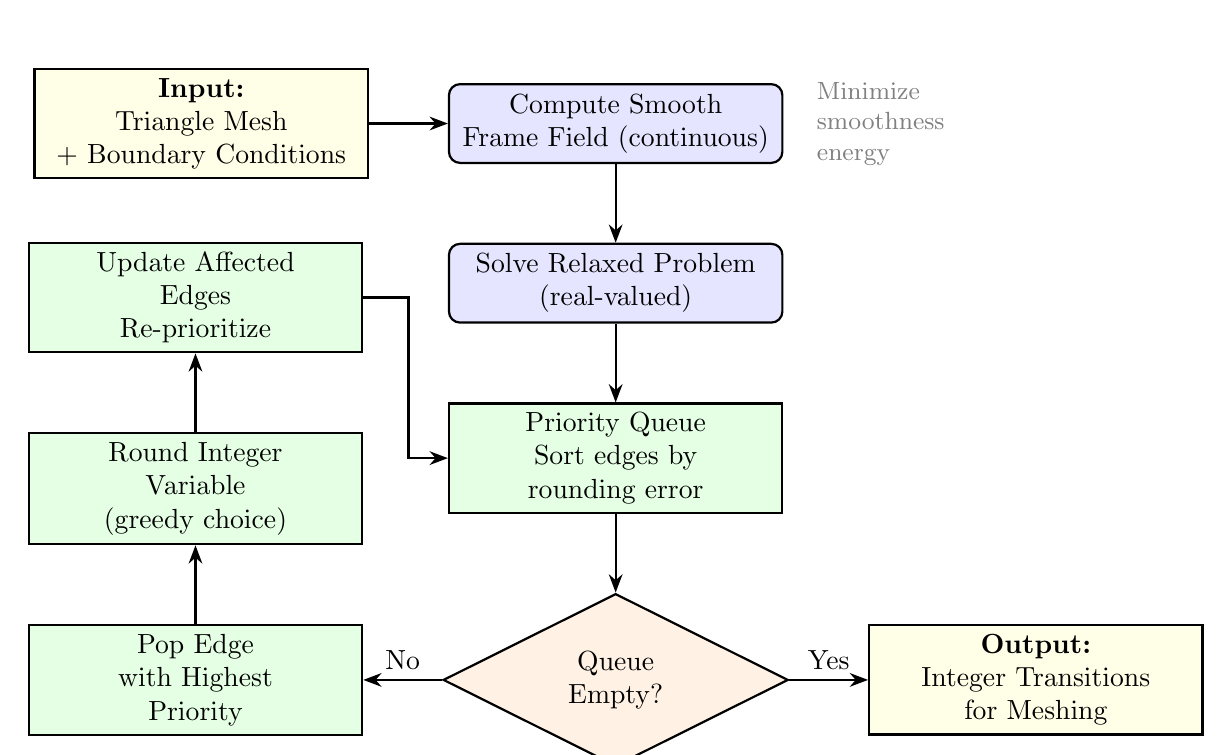
\begin{tikzpicture}[
    node distance = 1cm and 1cm,
    box/.style = {rectangle, rounded corners, draw=black, thick, fill=blue!10, 
                  text width=4cm, minimum height=1cm, align=center},
    process/.style = {rectangle, draw=black, thick, fill=green!10,
                      text width=4cm, minimum height=1cm, align=center},
    decision/.style = {diamond, draw=black, thick, fill=orange!10, aspect=2,
                       text width=2.5cm, align=center, inner sep=2pt},
    data/.style = {rectangle, draw=black, thick, fill=yellow!10,
                   text width=4cm, minimum height=0.8cm, align=center},
    arrow/.style = {-Stealth, thick}
]

% Input
\node[data] (input) {\textbf{Input:}\\Triangle Mesh\\+ Boundary Conditions};

% Step 1: Frame Field
\node[box, right=of input] (framefield) {Compute Smooth\\Frame Field (continuous)};

% Step 2: Relaxed Solution
\node[box, below=of framefield] (relaxed) {Solve Relaxed Problem\\(real-valued)};

% Step 3: Priority Queue
\node[process, below=of relaxed] (priority) {Priority Queue\\Sort edges by\\rounding error};

% Decision Loop
\node[decision, below=of priority] (decision) {Queue\\Empty?};

% Step 4: Pop Edge
\node[process, left=of decision] (pop) {Pop Edge\\with Highest\\Priority};

% Step 5: Round
\node[process, above=of pop] (round) {Round Integer\\Variable\\(greedy choice)};

% Step 6: Update
\node[process, above=of round] (update) {Update Affected\\Edges \\ Re-prioritize};

% Output
\node[data, right=of decision] (output) {\textbf{Output:}\\Integer Transitions\\for Meshing};

% Arrows
\draw[arrow] (input) -- (framefield);
\draw[arrow] (framefield) -- (relaxed);
\draw[arrow] (relaxed) -- (priority);
\draw[arrow] (priority) -- (decision);
\draw[arrow] (decision) -- node[above] {No} (pop);
\draw[arrow] (pop) -- (round);
\draw[arrow] (round) -- (update);
\draw[arrow] (decision) -- node[above] {Yes} (output);
\draw[arrow] (update) -| ([xshift=-0.5cm]priority.west) |- (priority);

% Annotations
\node[right=0.3cm of framefield, text width=2.5cm, align=left, font=\small\color{gray}] 
    {Minimize smoothness\\energy};
% \node[right=0.3cm of relaxed, text width=2.5cm, align=left, font=\small\color{gray}] 
%     {LP or QP\\relaxation};
% \node[right=0.3cm of round, text width=2.5cm, align=left, font=\small\color{gray}] 
%     {Locally optimal\\no backtracking};

\end{tikzpicture}
\caption{High-level workflow of the greedy mixed-integer solver.}
\label{fig:greedy_solver}
\end{figure}


Rather than rounding the first $k$ real valued variables to integers, the greedy rounding approch rounds one integer variable at a time. This is followed by an immediate update of the continous part treating the integers as constants. 

Let $\vec{x}^0$ be the continuous solution to the linear system and let $x_i$, $i \leq k$ be the variable which causes the smallest absolute error if we round it to the nearest integer. Then we set $x_i$ to this integer value. We solve the remaining variables $\vec{x}^1$ and continue to eliminate in eahc step that variable which cauess the least round-off error until we have an integer for all $x_1, \dots, x_k$.

To reduce the computational cost, we use a local Gauss-Seidel update rather than solving the full linear system after each rounding step. That means after after $x_i$ is rounded, we add all variables whose Gauss-Seidel update depends on $x_i$ to a priority queue. These elements correspond to the nonzero elements in row $A_i$. Now on each iteration, we pop the highest priority element from the queue, compute the local residuum 
\begin{equation}
    r_k = b_k - \sum_{j \neq n} A_{kj} x_j.
\end{equation}
If $|r_k| \geq \tau$, a small threshold, we update $x_k \leftarrow x_k - r_k / A_{kk}$ and push all variables which depend on $x_k$ back into the priority queue. This continues until the queue is empty. If the method does not converge in a reasonable number of iterations, we fall back to solving the full linear system. Figure \ref{fig:greedy_solver} illustrates the high-level workflow of this algorithm while Algorithm \ref{alg:greedy_solver} provides the detailed pseudocode. 



\begin{algorithm}
\caption{Greedy Mixed-Integer Solver}
\label{alg:greedy_solver}
\KwIn{System matrix $A$, right-hand side $b$, number of integer variables $k$, threshold $\tau$}
\KwOut{Solution vector $\vec{x}$ with integer values for $x_1, \ldots, x_k$}

\BlankLine

\tcp{Solve continuous relaxation}
Solve linear system $A\vec{x}^0 = b$ for all variables\;
$\text{rounded} \leftarrow \emptyset$\;

\BlankLine

\tcp{Round integer variables greedily}
\For{$i = 1$ \KwTo $k$}{
    \tcp{Find variable with minimum rounding error}
    $j \leftarrow \arg\min_{j \in \{1,\ldots,k\} \setminus \text{rounded}} |x_j^{i-1} - \text{round}(x_j^{i-1})|$\;
    
    \tcp{Round and fix variable}
    $x_j \leftarrow \text{round}(x_j^{i-1})$\;
    $\text{rounded} \leftarrow \text{rounded} \cup \{j\}$\;
    
    \BlankLine
    
    \tcp{Update affected continuous variables using Gauss-Seidel}
    \tcp{Q contains indices $m$ where $A_{mj} \neq 0$ (row $j$ has nonzero entry)}
    $Q \leftarrow \{ m : A_{mj} \neq 0 \}$\;
    
    \While{($Q$ is not empty) and (iteration count $<$ max\_iterations)}{
        $m \leftarrow Q.\text{pop}()$\;
        
        \tcp{Compute local residual}
        $r_m \leftarrow b_m - \sum_{n} A_{mn} x_n$\;
        
        \If{$|r_m| \geq \tau$}{
            \tcp{Update variable}
            $x_m \leftarrow x_m - r_m / A_{mm}$\;
            
            \tcp{Add dependent variables to queue}
            \For{each $n$ where $A_{nm} \neq 0$}{
                $Q.\text{push}(n)$\;
            }
        }
    }
}

\BlankLine

\Return{$\vec{x}$}\;
\end{algorithm}



\subsection{Frame Field Generation}
In this section we introduce the mathematical formulation and implementation details for generating a smooth frame field over a given triangular mesh. 


\subsubsection{Mathematical Formulation}
A frame field is a $N$-symmetry direction field (Ray et al. 2008b) where at each point in the domain, $N$ directions are defined that are symmetric under rotation by $2\pi/N$ around the point of interest. For quadrilateral meshing, we are interested in 4-symmetry frame fields, or cross fields, where $N=4$. For the rest of the project, we will take $N = 4$. The frame field is represented by an angle-field $\theta: F \mapsto \mathbb{R}$ which assigns an angle $\theta_f$ to each face $f \in F$ of the triangular mesh and a period-jump field $p: E \mapsto \mathbb{Z}$ which assigns an integer period-jump $p_e$ to each edge $e \in E$ of the mesh.  

The idea is that for each face $f$, we can define a local frame of reference by rotating a reference edge $e$ along the $x$-axis. Then the four directions of the frame at face $f$ are given by rotating this reference edge by angles $\theta_f + k \cdot \pi/2$ for $k = 0, 1, 2, 3$. This is visualized in Figure \ref{fig:frame_field_combined} \ref{sub@fig:frame_field}. The period-jump field $p_e$ determines which direction in face $f_1$ corresponds to which direction in the adjacent face $f_2$ across edge $e$. Specifically, the direction in face $f_2$ that aligns with the reference edge is given by $\theta_{f_2} + p_e \cdot \pi/2$. This relationship is illustrated in Figure \ref{fig:frame_field_combined} \ref{sub@fig:period_jump}.

\begin{figure}[H]
\centering
\begin{minipage}[b]{0.48\textwidth}
\centering
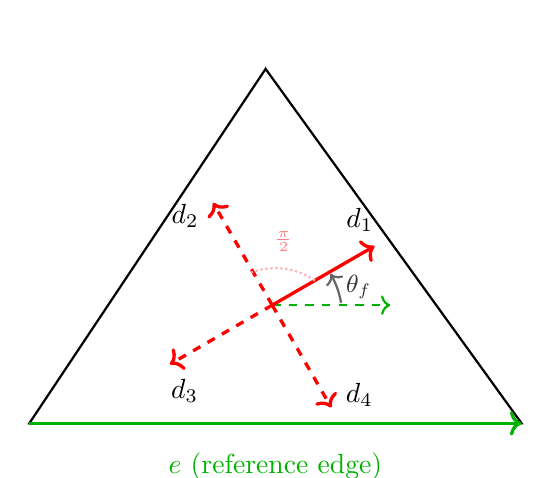
\begin{tikzpicture}[scale=2.5]
    % Define triangle vertices
    \coordinate (A) at (0, 0);
    \coordinate (B) at (2.5, 0);
    \coordinate (C) at (1.2, 1.8);
    
    % Calculate centroid
    \coordinate (center) at (barycentric cs:A=1,B=1,C=1);
    
    % Draw triangle
    \draw[thick] (A) -- (B) -- (C) -- cycle;
    
    % Highlight reference edge e (aligned with x-axis)
    \draw[->, very thick, green!70!black] (A) -- (B);
    \node[below, green!70!black] at (1.25, -0.1) {$e$ (reference edge)};
    
    % Draw x-axis reference at center
    \draw[->, thick, green!70!black, dashed, line width=0.8pt] (center) -- ++(0.6, 0);
    
    % Define rotation angle theta (30 degrees for visualization)
    \def\thetaAngle{30}
    
    % Draw d1 direction (rotated by theta from x-axis)
    \draw[->, thick, red, line width=1.2pt] (center) -- ++(\thetaAngle:0.6);
    \node[above left, black] at ([shift={(\thetaAngle:0.65)}]center) {$d_1$};
    
    % Draw rotation arc for theta
    \draw[->, black!60, thick] ([shift={(2:0.35)}]center) arc (10:\thetaAngle:0.45);
    \node[black!80, font=\small] at ([shift={(12:0.45)}]center) {$\theta_f$};
    
    % Draw d2, d3, d4 directions (rotated by pi/2 increments)
    \draw[->, thick, red, line width=1.2pt, dashed] (center) -- ++(\thetaAngle+90:0.6);
    \node[below left, black] at ([shift={(\thetaAngle+90:0.65)}]center) {$d_2$};
    
    \draw[->, thick, red, line width=1.2pt, dashed] (center) -- ++(\thetaAngle+180:0.6);
    \node[below right, black] at ([shift={(\thetaAngle+180:0.65)}]center) {$d_3$};
    
    \draw[->, thick, red, line width=1.2pt, dashed] (center) -- ++(\thetaAngle+270:0.6);
    \node[above right, black] at ([shift={(\thetaAngle+270:0.65)}]center) {$d_4$};
    
    % Draw rotation arcs between directions
    \draw[red!30, densely dotted, thick] ([shift={(\thetaAngle :0.25)}]center) arc (\thetaAngle+25:\thetaAngle+90-10:0.35);
    \node[red!50, font=\scriptsize] at ([shift={(\thetaAngle+50:0.33)}]center) {$\frac{\pi}{2}$};
    
\end{tikzpicture}
\subcaption{}
\label{fig:frame_field}
\end{minipage}
\hfill
\begin{minipage}[b]{0.48\textwidth}
\centering
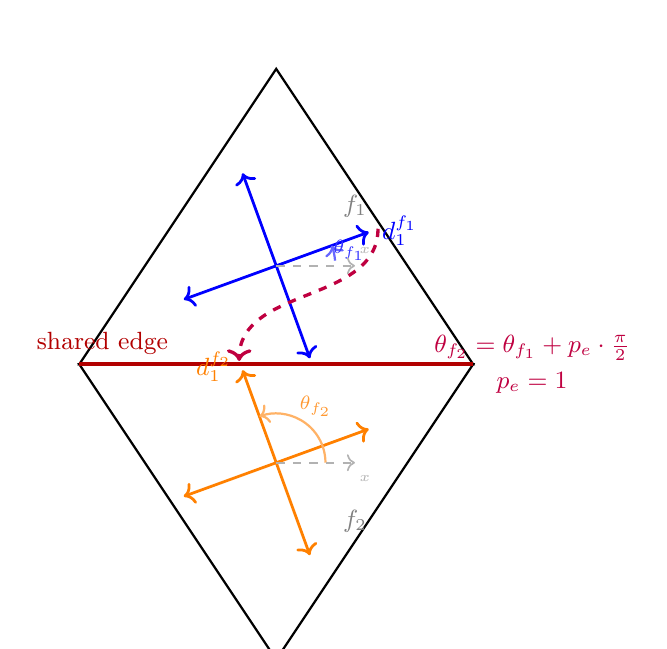
\begin{tikzpicture}[scale=2.5]
    % Define vertices for two adjacent triangles
    \coordinate (A) at (0, 0);
    \coordinate (B) at (2, 0);
    \coordinate (C) at (1, 1.5);
    \coordinate (D) at (1, -1.5);
    
    % Calculate centroids
    \coordinate (center1) at (barycentric cs:A=1,B=1,C=1);
    \coordinate (center2) at (barycentric cs:A=1,B=1,D=1);
    
    % Draw triangles
    \draw[thick] (A) -- (B) -- (C) -- cycle;
    \draw[thick] (A) -- (B) -- (D) -- cycle;
    
    % Highlight shared edge
    \draw[very thick, red!70!black, line width=1.5pt] (A) -- (B);
    \node[above left, red!70!black, font=\small] at (0.5, 0.0) {shared edge};
    
    % Face 1 (top triangle)
    \def\thetaOne{20}
    \def\periodJump{1}  % p_e = 1
    
    % Frame directions for face 1
    \draw[->, thick, blue, line width=1pt] (center1) -- ++(\thetaOne:0.5);
    \node[right, blue, font=\small] at ([shift={(\thetaOne:0.52)}]center1) {$d_1^{f_1}$};
    
    \draw[->, thick, blue, line width=1pt] (center1) -- ++(\thetaOne+90:0.5);
    \draw[->, thick, blue, line width=1pt] (center1) -- ++(\thetaOne+180:0.5);
    \draw[->, thick, blue, line width=1pt] (center1) -- ++(\thetaOne+270:0.5);
    
    % Label for theta_1
    \draw[->, blue!60, thick] ([shift={(5:0.3)}]center1) arc (5:\thetaOne:0.3);
    \node[blue!80, font=\scriptsize] at ([shift={(12:0.38)}]center1) {$\theta_{f_1}$};
    
    % Face 2 (bottom triangle)
    \def\thetaTwo{110}  % theta_2 = theta_1 + p_e * pi/2 = 20 + 1*90 = 110
    
    % Frame directions for face 2
    \draw[->, thick, orange, line width=1pt] (center2) -- ++(\thetaTwo:0.5);
    \node[left, orange, font=\small] at ([shift={(\thetaTwo:0.52)}]center2) {$d_1^{f_2}$};
    
    \draw[->, thick, orange, line width=1pt] (center2) -- ++(\thetaTwo+90:0.5);
    \draw[->, thick, orange, line width=1pt] (center2) -- ++(\thetaTwo+180:0.5);
    \draw[->, thick, orange, line width=1pt] (center2) -- ++(\thetaTwo+270:0.5);
    
    % Label for theta_2
    \draw[->, orange!60, thick] ([shift={(0:0.25)}]center2) arc (0:\thetaTwo:0.25);
    \node[orange!80, font=\scriptsize] at ([shift={(55:0.35)}]center2) {$\theta_{f_2}$};
    
    % Show period jump relationship
    \draw[->, thick, purple, dashed, line width=1.2pt] ([shift={(\thetaOne:0.55)}]center1) 
          to[out=-90, in=90] ([shift={(\thetaTwo:0.55)}]center2);
    \node[purple, font=\small, align=center] at (2.3, 0) {$\theta_{f_2} = \theta_{f_1} + p_e \cdot \frac{\pi}{2}$\\[2pt]$p_e = 1$};
    
    % Label faces
    \node[gray, font=\small\itshape] at ([shift={(0.4,0.3)}]center1) {$f_1$};
    \node[gray, font=\small\itshape] at ([shift={(0.4,-0.3)}]center2) {$f_2$};
    
    % Draw x-axis reference (dashed)
    \draw[->, dashed, gray!60, line width=0.6pt] (center1) -- ++(0.4, 0);
    \draw[->, dashed, gray!60, line width=0.6pt] (center2) -- ++(0.4, 0);
    \node[gray!60, font=\tiny] at ([shift={(0.45,0.08)}]center1) {$x$};
    \node[gray!60, font=\tiny] at ([shift={(0.45,-0.08)}]center2) {$x$};
    
\end{tikzpicture}
\subcaption{}
\label{fig:period_jump}
\end{minipage}
\caption{Frame field visualization. (a) The reference edge $e$ is aligned with the $x$-axis. The frame at face $f$ consists of four directions obtained by rotating the $x$-axis by angles $\theta_f, \theta_f + \frac{\pi}{2}, \theta_f + \pi, \theta_f + \frac{3\pi}{2}$. (b) The frame field in face $f_2$ is related to face $f_1$ by $\theta_{f_2} = \theta_{f_1} + p_e \cdot \frac{\pi}{2}$, where $p_e = 1$ causes a $90^\circ$ rotation.}
\label{fig:frame_field_combined}
\end{figure}



\subsubsection{Constructing a Smooth Frame Field}
The smoothness of a unit frame field can be measured by the angular difference between faces:
\begin{equation}\label{eq:smooth_energy}
    E_\text{smooth} = \sum_{e_{ij} \in E} \left(\theta_i + \kappa_{ij} + \frac{2\pi}{N} p_{ij} - \theta_j\right)^2,
\end{equation}
where $\theta_i$, and $\theta_j$ are the angles of trangle $i$ and $j$ to it's respective reference edge, $\kappa_{ij} \in (-\pi, \pi]$ is the angle between the reference edges of triangles $i$ and $j$, $p_{ij}$ is the integer period-jump across edge $e_{ij}$, and $N=4$ for quadrilateral meshing.

The cross field index of a vertex $v$ is defined as:
\begin{equation}
    I(v) = I_0(v) + \sum_{e_{ij} \in \text{star}(v)} \frac{p_{ij}}{4},
\end{equation}
where $I_0(v)$ is the initial index determined by the geometry of the mesh 
\begin{equation}
    I_0(v) =  \frac{1}{2\pi} \left( A_d(v) + \sum_{e_{ij} \in \text{star}(v)} \kappa_{ij} \right),
\end{equation}
where $A_d(v)$ is the angle defect at vertex $v$ and $\text{star}(v)$ is the set of edges incident to vertex $v$. Ray et. al. (2008b) show that vertices with non-zero index correspond to singularities in the frame field which will later correspond to irregular vertices in the quadrilateral mesh. The index will be an multiple of $1/4$ and determine the valence of the irregular vertex in the quad mesh e.g., an index of $+1/4$ corresponds to a vertex with valence 3 while an index of $-1/4$ corresponds to a vertex with valence 5.

\subsubsection{Finding a Smooth Frame Field}
The problem we wish to solve is given a triangular mesh $M$ and a subset of faces $F_c \subset F$ with constrained direction $\theta_i = \hat{\theta}_i$ for $i \in F_c$, we search for a smooth frame field by minimizing the energy given by equation \ref{eq:smooth_energy}. That is, we wish to solve for $\theta_i$ and $p_{ij}$, which minimize $E_\text{smooth}$ subject to the constraints $\theta_i = \hat{\theta}_i$ for $i \in F_c$. This is a mixed-integer problem since $\theta_i$ are real-valued while $p_{ij}$ are integers.

To reduce the problem space, we can take advantage of the invaraiance under rotation of the frame field. Following the work of Bommes et al. (2009), the minimization problem can be mind unique by fixing one period jump variable to zero per triangle. In order to not change the value of the energy, we take care not to fix edges whose dual paths connect two constrained faces, or closes loops. To generate a valid set of edges whose period jumps may be fixed, we construct a Dijkstra tree over the dual graph of the triangular mesh, starting from the constrained faces. A visualization of this process is shown in Figure \ref{fig:dijkstra_tree}. 


\begin{figure}
    \centering
    \includegraphics[width=0.5\textwidth,height=\textwidth,keepaspectratio]{../frame_field/output/forests/triangulation_forest_simple-square.png}
    \caption{Constrained faces are highlighted in red with a Dijkstra tree spanning along the dual graph. Importantly we see that the trees do not loop or connect to trees from other constrained faces. Edges in the primal graph whose dual edges are part of the Dijkstra tree may have their period jumps fixed to zero without changing the energy of the frame field.}
    \label{fig:dijkstra_tree}
\end{figure}


\subsubsection{Implementation Details}
To implement the frame field generation, we first construct the Dijkstra tree to identify edges whose period jumps can be fixed. We then set up the minimization problem by taking the derivative of the energy function with respect to each variable, leading to a system of linear equations for the real-valued variables $\theta$ and integer constraints for the period jumps $p$. The resulting equations are as follows:
\begin{equation}
    \begin{aligned}
    \frac{\partial E_\text{smooth}}{\partial \theta_k} &= \sum_{e_{kj} \in \text{star}(v)} 2 \left(\theta_k + \kappa_{kj} + \frac{\pi}{2} p_{kj}  - \theta_j \right) = 0, \\
    \frac{\partial E_\text{smooth}}{\partial p_{ij}} &= \pi\left( \theta_i + \kappa_{ij} + \frac{\pi}{2} p_{ij} - \theta_j \right) = 0. 
    \end{aligned}
\end{equation}
For all variables that are not fixed, we assemble a row in a single matrix that we pass to the greedy mixed-integer solver described earlier. The solver returns the optimal $\theta$ and $p$ values which define the smooth frame field over the triangular mesh adhering to the user-defined constraints on $F_c$.




\subsection{Quadrilateral Mesh Extraction}






\clearpage

% --- RESULTS ---
\section{Results}


\clearpage

% --- DISCUSSION ---
\section{Discussion}


\clearpage

% --- CONCLUSION ---
\section{Conclusion}



% --- REFERENCES ---

\clearpage 
% --- APPENDIX ---
\appendix
\section{Julia Code Listings}
\label{app:code}

All code used in this project is available at the following GitHub repository: \url{https://github.com/MarvynBailly/Structured-Grid-Generation-via-Frame-Fields}.

\section{Reference Paper}
\label{app:paper}

The following pages contain the full text of Bommes et al. %(2009) \cite{bommes2009mixed}.

% Include the PDF file (place bommes2009.pdf in the same directory)
% \includepdf[pages=-,pagecommand={},width=\textwidth]{Bommes-2009-MIQ.pdf}

\end{document}